\chapter{Cap\'{\i}tulo 3: Modelo de regresi\'{o}n ZOIP con efectos fijos}\label{cap3}
%{\Huge \textbf{Modelo de regresi\'{o}n ZOIP con efectos fijos\\}}
%Los datos obtenidos a partir de variables medidas bajo porcentajes, tasas y proporciones, son llamados datos proporcionales y estos se encuentran ubicados por lo general en el intervalo (0,1), sin embargo existen casos de este tipo de variables pueden dar resultados de cero y/o uno, representando la ausencia o presencia total de la caracter\'{\i}stica medida a partir de una variable, este tipo de datos son conocidos como datos proporcionales inflados con ceros y/o unos, existen diferentes distribuciones que explican estos datos, tales como la distribuci\'{o}n beta inflada con ceros o unos \citep{Ospina2} o de una manera m\'{a}s general la distribuci\'{o}n ZOIP (Zeros Ones inflated Proportional) que busca reunir la distribuci\'{o}n simplex y beta bajo diferentes parametrizaciones en una sola distribuci\'{o}n.\\

En muchos casos de estudios es factible preguntarse c\'{o}mo puede ser explicada una variable aleatoria proveniente de datos proporcionales a partir de diferentes variables, es decir un modelo de regresi\'{o}n para datos proporcionales, el modelo m\'{a}s conocido en la literatura para este tipo de datos es la regresi\'{o}n beta, donde \cite{Paolino1} estima mediante m\'{a}xima verosimilitud modelos de variables dependientes de una distribuci\'{o}n beta, utilizando la parametrizaci\'{o}n original, m\'{a}s adelante  \cite{Ferrari2} reparametrizan la distribuci\'{o}n e introducen la regresi\'{o}n beta bajo esta nueva parametrizaci\'{o}n, m\'{a}s adelante en el paquete \pkg{betareg} de \proglang{R} \citep{Zeileis1} implementan dicha regresi\'{o}n. Por otro parte \cite{Stasinopoulos2} tambi\'{e}n realizan otra reparametrizaci\'{o}n de la distribuci\'{o}n beta original, basado en par\'{a}metros como la media y la dispersi\'{o}n, adem\'{a}s introducen un modelo de regresi\'{o}n beta basado en dicha distribuci\'{o}n y lo implementan en el paquete \pkg{gamlss} de \proglang{R}, sin embargo existen otros tipos de regresiones basadas en otras distribuciones, como la regresi\'{o}n simplex, que se encuentra bajo la distribuci\'{o}n para datos proporcionales simplex \citep{Barndorff1}, dicha regresi\'{o}n fue realizada por \cite{Qiu1} e implementada en el paquete \pkg{simplexreg} de \proglang{R} \citep{Zhang1}.\\

Sin embargo los anteriores modelos de regresi\'{o}n son realizados para datos proporcionales no inflados con ceros o unos, es por esto que \cite{Ospina1} realizan un modelo de regresi\'{o}n inflado con cero o con uno, no con ambos, bajo la distribuci\'{o}n beta inflada de \cite{Ospina2} con parametrizaci\'{o}n \cite{Ferrari2}, de igual manera \cite{Stasinopoulos2} implementan los modelos de regresi\'{o}n beta inflados en ceros y/o unos, y se encuentran implementados en el paquete \pkg{gamlss} de \proglang{R} \citep{Stasinopoulos1}, sin embargo para la utilizaci\'{o}n del modelo de regresi\'{o}n inflado solo con ceros o unos o con ambos, se deben utilizar funciones distintas dentro del paquete para ajustar los tres diferentes modelos de regresi\'{o}n. Adem\'{a}s no existen paquetes en \proglang{R} que logren ajustar un modelo de regresi\'{o}n beta inflado con ceros y/o unos bajo las parametrizaciones originales y de \cite{Ferrari2}, por otra parte a pesar de que existen desarrollos te\'{o}ricos sobre el modelo de regresi\'{o}n simplex inflado con ceros y/o unos \citep{Galvis1}, no existe un paquete en \proglang{R} que permita realizar un ajuste sobre dicho modelo de regresi\'{o}n.\\

Es por esto que en este trabajo se implementa de manera te\'{o}rica y de forma pr\'{a}ctica mediante el paquete \pkg{ZOIP} en el sistema de computaci\'{o}n \proglang{R} \citep{R} y disponible en el repositorio web \verb|GitHub|, un modelo de regresi\'{o}n para datos proporcionales inflados con ceros y/o unos (Modelo de regresi\'{o}n ZOIP) que permita mediante una misma funci\'{o}n ajustar modelos en diferentes distribuciones para datos proporcionales y en diferentes parametrizaciones.\\

Este cap\'{\i}tulo se encuentra organizado de la siguiente manera: primero se presenta el modelo de regresi\'{o}n ZOIP que es basado en la distribucion ZOIP visto en el capitulo anterior y su debida estimaci\'{o}n, mediante maxima verosimilitud, en la siguiente secci\'{o}n se presenta la implementaci\'{o}n del modelo de regresi\'{o}n ZOIP en el paquete \pkg{ZOIP} de \proglang{R} y por \'{u}ltimo se presenta unas aplicaciones a datos simulados y a datos reales.

%%%%%%%%%%%%%%%%%%%%%%%%%%%%%%%%%%%%%%%%%%%%%%%%%%%%%%%%%%%%%%%%%%%%%%%%%%%%%%%%%%%%%%%%%%%%%%%%%%%%%%%%%%%%%%%%%%%%%%%%%%%%%%%%%%%%%%%%%%%%%%%%%%%%%%%%%%%%%%%%%%

\section{Modelo de regresi\'{o}n ZOIP}

Una clase general de modelos de regresi\'{o}n ZOIP puede definirse como sigue. Sea $y_1, y_2,\ldots, y_n$ variables aleatorias independientes tal que cada $y_i$, para $i=1,\ldots, n$, tiene funci\'{o}n de densidad de probabilidad \eqref{eq_Dist_ZOIP} con par\'{a}metros $\mu = \mu_i$, $\sigma=\sigma_i$,  $p_0=p_{0i}$, y $p1=p_{1i}$. Se asume que $\mu_i$, $\sigma_i$, $p_{0i}$ y $p_{1i}$ se definen como

\begin{equation}
\begin{split}
&h_1(\mu_{i})=\mathbf{x}_{i1}^{\top} \boldsymbol{\beta}_1,\\
&h_2(\sigma_{i})=\mathbf{x}_{i2}^{\top} \boldsymbol{\beta}_2,\\
&h_3(p_{0i})=\mathbf{x}_{i3}^{\top} \boldsymbol{\beta}_3,\\
&h_4(p_{1i}) =\mathbf{x}_{i4}^{\top} \boldsymbol{\beta}_4
\end{split}
\label{eq_reg}
\end{equation}

donde $\mathbf{x}_{i1}=(x_{i11}, x_{i12},\ldots, x_{i1k_1})$, $\mathbf{x}_{i2}=(x_{i21}, x_{i22},\ldots, x_{i2k_2})$, \\
$\mathbf{x}_{i3}=(x_{i31}, x_{i32},\ldots, x_{i1k_3})$ y $\mathbf{x}_{i4}=(x_{i41}, x_{i42},\ldots, x_{i1k_4})$, son vectores de covariables conocidos de dimensi\'{o}n $k_1$, $k_2$, $k_3$ y $k_4$ respectivamente, $\boldsymbol{\beta}_1=(\beta_{11}, \beta_{12},\ldots, \beta_{1k_1})$, $\boldsymbol{\beta}_2=(\beta_{21}, \beta_{22},\ldots, \beta_{2k_2})$, $\boldsymbol{\beta}_3=(\beta_{31}, \beta_{32},\ldots, \beta_{3k_3})$ y $\boldsymbol{\beta}_4=(\beta_{41}, \beta_{42},\ldots, \beta_{4k_4})$ son vectores de par\'{a}metros de regresi\'{o}n desconocidos. Adem\'{a}s se asume que las funciones de enlace $h_1(\cdot)$, $h_2(\cdot)$, $h_3(\cdot)$ y $h_4(\cdot)$ son conocidas y apropiadas para mapear de los reales a los valores admisibles del par\'{a}metro, ademas son funciones estrictamente mon\'{o}tonas y doblemente diferenciables. Las posibles funciones para el par\'{a}metro $\mu$ y $\sigma$ son logit, probit, clog-log, o log dependiendo de la parametrizaci\'{o}n,  para los par\'{a}metros de inflaci\'{o}n $p_0$ y $p_1$ son posibles funciones de enlace como logit, probit, clog-log. Estudios sobre funciones enlace mal especificadas sobre modelos de regresi\'{o}n beta se encuentran en \cite{andrade07}.

\subsection{Inferencia estad\'{\i}stica}

Para estimar los par\'{a}metros del modelo de regresi\'{o}n ZOIP, se usar\'{a} el m\'{e}todo de m\'{a}xima verosimilitud. La funci\'{o}n de verosimilitud para $\boldsymbol{\theta}=(\boldsymbol{\beta_1}^{\top},\boldsymbol{\beta_2}^{\top},\boldsymbol{\beta_3}^{\top}, \boldsymbol{\beta_4}^{\top})^{\top}$, basado en una muestra de observaciones independientes, es de la forma:

\begin{equation}
L(\boldsymbol{\theta})=\prod_{i=1}^{n}g(\mathbf{y}_i;\mu_i,\sigma_i,p_{0i},p_{1i}) 
\label{F_likel}
\end{equation}

%\[
%\ell(\boldsymbol{\theta})=\sum_{i=1}^{n}{\ell_i(\mu_i,\sigma_i,p_{0i},p_{1i}) }
%\]

donde para el caso de ZOIP-beta original $\mu_i=p_i$, $\sigma_i=q_i$; si la distribuci\'{o}n ZOIP-beta fuese con parametrizaci\'{o}n de \cite{Ferrari2} el \'{u}nico par\'{a}metro que cambiar\'{\i}a es $\sigma_i=\phi_i$, el resto de los par\'{a}metros no tendr\'{\i}an modificaciones seg\'{u}n su parametrizaci\'{o}n o distribuci\'{o}n.\\

La funci\'{o}n de verosimilitud definida en \eqref{F_likel} al aplicar logaritmo natural se obtiene la funci\'{o}n de log verosimilitud definida como:
\[
\ell(\boldsymbol{\theta})=\ell_1(\boldsymbol{\beta_3})+\ell_2(\boldsymbol{\beta_4})+\ell_3(\boldsymbol{\beta_1},\boldsymbol{\beta_2})
\]
\\
Note que la funci\'{o}n de verosimilitud es factorizada en tres t\'{e}rminos, dos de ellos del componente discreto y uno compuesto por $\boldsymbol{\beta_1}$ y $\boldsymbol{\beta_2}$ del componente continuo, por tanto los par\'{a}metros son separables \citep{Pace1}, as\'{\i} la m\'{a}xima verosimilitud puede ser tratada por separado y por lo tanto:\\
\begin{align*}
\begin{split}
	\ell_1(\boldsymbol{\beta_3}) &= \sum_{i=1}^{n}{p_{0i}^{S_0(y_i)}(1-p_{0i})^{1-S_0(y_i)}}
\end{split}\\
\begin{split}
	\ell_2(\boldsymbol{\beta_4}) &= \sum_{i=1}^{n}{p_{1i}^{S_1(y_i)}(1-p_{1i})^{1-S_1(y_i)}}
\end{split}\\
\begin{split}
	\ell_3(\boldsymbol{\beta_1},\boldsymbol{\beta_2}) &= \sum_{i=1:y_i \in (0,1)}^{n}{f(y_i;\mu_i,\sigma_i)} 
\end{split}
\end{align*}

Con
\[
S_j(y_i)=
\begin{cases}
1 & \text{si}\ y_i=j\\
0 & \text{si}\ y_i\neq j\\
\end{cases}
\quad ; \quad j=1,2
\]
\\
Con $p_{0i}=h_3^{-1}(\mathbf{x}_{i3}^{\top} \boldsymbol{\beta}_3)$, $p_{1i}=h_4^{-1}(\mathbf{x}_{i4}^{\top} \boldsymbol{\beta}_4)$, $\mu_i=h_1^{-1}(\mathbf{x}_{i1}^{\top} \boldsymbol{\beta}_1)$ y $\sigma_i=h_2^{-1}(\mathbf{x}_{i2}^{\top} \boldsymbol{\beta}_2)$ como se definio en \eqref{eq_reg}. La funcion de verosimilitud depende de tres terminos, el primero depende de  $\boldsymbol{\beta}_3$ (componente discreto para inflaci\'{o}n en cero), el segundo de $\boldsymbol{\beta}_4$ (componente discreto para explicar la inflaci\'{o}n en uno) y el tercero depende de $(\boldsymbol{\beta}_1,\boldsymbol{\beta}_2)$ (Componentes para explicar la parte continua), por lo tanto los par\'{a}metros son separables y la inferencia de m\'{a}xima verosimilitud para $\boldsymbol{\beta}_1$ y $\boldsymbol{\beta}_2$ se puede hacer por separado de la de $\boldsymbol{\beta}_3$ y $\boldsymbol{\beta}_4$, como si conociera a $\boldsymbol{\beta}_3$ y $\boldsymbol{\beta}_4$ y viceversa. \citep{Ospina1}.\\

No existen expresiones que den una soluci\'{o}n cerrada anal\'{\i}ticamente para encontrar los m\'{a}ximos de las  funciones de log verosimilitudes descritas anteriormente, para as\'{\i} hallar los estimadores de m\'{a}xima verosimilitud de los par\'{a}metros de regresi\'{o}n de cada uno de los componentes de la distribuci\'{o}n ZOIP.  Por lo que es necesario utilizar algoritmos de optimizaci\'{o}n no lineal como el m\'{e}todo de Newton-Raphson o Fisher's scoring, para nuestro caso utilizaremos el algoritmo de optimizaci\'{o}n dado por la funci\'{o}n \code{nlminb} o \code{optim} del paquete \code{stats} de \proglang{R} e implementado en el paquete \pkg{ZOIP} de \proglang{R} para el modelo de regresi\'{o}n ZOIP.

%%%%%%%%%%%%%%%%%%%%%%%%%%%%%%%%%%%%%%%%%%%%%%%%%%%%%%%%%%%%%%%%%%%%%%%%%%%%%%%%%%%%%%%%%%%%%%%%%%%%%%%%%%%%%%%%%%%%%%%%%%%%%%%%%%%%%%%%%%%%%%%%%%%%%%%%%%%%%%%%%%

\section{Modelo de regresi\'{o}n ZOIP en el Paquete \pkg{ZOIP}}

En esta secci\'{o}n presentaremos como el paquete \pkg{ZOIP} realizado en \proglang{R} ajusta un modelo de regresi\'{o}n ZOIP con efectos fijos, v\'{\i}a m\'{a}xima verosimilitud.

%\subsection{Instalaci\'{o}n}
%
%La versi\'{o}n m\'{a}s actualizada del paquete \pkg{ZOIP} se encuentra ubicada en \verb|GitHub|, el cual es un alojamiento de repositorios Git, para obtener dicha versi\'{o}n es necesario ejecutar el siguiente c\'{o}digo que instala el devtools que es necesario para descargar el paquete \pkg{ZOIP}.
%
%\begin{verbatim}
%if (!require('devtools')) install.packages('devtools')
%devtools::install_github('jucdiaz/ZOIP', force=TRUE)
%require(ZOIP)  # Carga el paquete
%\end{verbatim}

\subsection{Funci\'{o}n RM.ZOIP}

La funci\'{o}n \code{RM.ZOIP} estima los par\'{a}metros de un modelo de regresi\'{o}n ZOIP con y sin covariables v\'{\i}a m\'{a}xima verosimilitud utilizando el optimizador \code{nlminb} o \code{optim}. La estructura de la funci\'{o}n \code{RM.ZOIP} es la siguiente:

\begin{verbatim}
RM.ZOIP(formula.mu, formula.sigma = ~1, formula.p0 = ~1, 
    formula.p1 = ~1, data, link = c("identity", "identity", 
        "identity", "identity"), family = "R-S", optimizer = "nlminb")
\end{verbatim}

Los argumentos de la funci\'{o}n \code{RM.ZOIP} son:

\begin{itemize}[noitemsep, nolistsep]

\item \code{formula.mu}: Formula que define la funci\'{o}n de regresi\'{o}n para el par\'{a}metro $\mu$, Un valor posible es \code{y $\sim$ x1 + x2}, es necesario definir la variable respuesta (y).
\item \code{formula.sigma}: Formula que define la funci\'{o}n de regresi\'{o}n para el par\'{a}metro $\sigma$, Un valor posible es \code{$\sim$ x1}. Por defecto \code{$\sim$ 1}.
\item \code{formula.p0}: Formula que define la funci\'{o}n de regresi\'{o}n para el par\'{a}metro $p_0$, Un valor posible es \code{$\sim $x1}. Por defecto \code{$\sim $1}.
\item \code{formula.p1}: Formula que define la funci\'{o}n de regresi\'{o}n para el par\'{a}metro $p_1$, Un valor posible es \code{$\sim $x1}. Por defecto \code{$\sim $1}.
\item \code{data}: es el conjunto de datos en formato \code{data.frame} donde debe contener las nombres de las columnas tal cual como est\'{a}n en las f\'{o}rmulas.
\item \code{family}: Elecci\'{o}n de la parametrizaci\'{o}n de la distribuci\'{o}n beta o distribuci\'{o}n deseada en la parte continua de la distribuci\'{o}n ZOIP, si toma el valor de \code{``R-S''} se utilizara la distribuci\'{o}n beta con parametrizaci\'{o}n  \cite{Stasinopoulos2}, si toma el valor de \code{``F-C''} se utilizara la distribuci\'{o}n beta parametrizaci\'{o}n \cite{Ferrari2}, el valor de \code{``Original''} se utilizara la distribuci\'{o}n beta con parametrizaci\'{o}n original, \code{``Simplex''} Utilizara la distribuci\'{o}n simplex.
\item \code{link}: Es un vector con las funciones enlace adecuadas para cada par\'{a}metro a estimar de acuerdo a las opciones escogidas en los par\'{a}metros de familia y formula. Si el modelo de regresi\'{o}n no posee covariables se debe utilizar como funci\'{o}n enlace la opci\'{o}n \code{identity}, independientemente del valor escogido en familia, opciones posibles son \code{logit}, \code{log}. Por defecto \code{link=c(``identity'',``identity'',``identity'',``identity'')}.
\item \code{optimizer}: Elecci\'{o}n del optimizador, utilizado para encontrar la convergencia de la m\'{a}xima verosimilitud. se puede elegir el valor de \code{``nlminb''} o \code{``optim''}. Por defecto \code{``nlminb''}
\end{itemize}

En el siguiente ejemplo nos concentraremos en el ajuste de un modelo regresi\'{o}n ZOIP, para ello se mostrar\'{a} el c\'{o}digo utilizado y la salida de la funci\'{o}n \code{RM.ZOIP}, para una variable aleatoria simulada de una distribuci\'{o}n ZOIP-beta con parametrizaci\'{o}n \cite{Stasinopoulos2} y dos covariables simuladas a partir de una distribuci\'{o}n uniforme entre cero y uno, el tama\~{n}o de la muestra simulada es 1000. Esto replicando exactamente uno de los casos de simulaci\'{o}n vistos en la pr\'{o}xima secci\'{o}n.\\

Primero se simula la variable respuesta a partir de la funci\'{o}n \code{rZOIP} con los debidos valores de los par\'{a}metros para cada observaci\'{o}n, y las covariables.

\begin{verbatim}
library(ZOIP)
n <- 1000
x1 <- runif(n)
x2 <- runif(n)

c1 <- 0.2
c2 <- -1
mu_i <- inv.logit(c1 + c2 * x1)

b1 <- 0.3
b2 <- 3
b3 <- 0.9
sigma_i <- inv.logit(b1 + b2 * x1 + b3 * x2)
\end{verbatim}
\begin{verbatim}
d1 <- 0.07
p0_i <- rep(d1, n)

e1 <- 0.02
e2 <- -4
p1_i <- inv.logit(e1 + e2 * x2)

param <- cbind(mu_i, sigma_i, p0_i, p1_i)
y_i <- apply(param, 1, function(x)
{
    rZOIP(1, mu = x[1], sigma = x[2], p0 = x[3], p1 = x[4], 
        family = "R-S")
})

data <- as.data.frame(cbind(y_i, x1, x2))

link <- c("logit", "logit", "identity", "logit")
mod <- RM.ZOIP(formula.mu = y_i ~ x1, formula.sigma = ~x1 + 
    x2, formula.p0 = ~1, formula.p1 = ~x2, data = data, 
    link = link, family = "R-S")

mod
\end{verbatim}

Los resultados obtenidos se muestran a continuaci\'{o}n.

\begin{verbatim}
## Call:
## RM.ZOIP(formula.mu = y_i ~ x1, formula.sigma = ~x1 + x2, formula.p0 = ~1, 
##     formula.p1 = ~x2, data = data, link = link, family = "R-S")
## 
##  Results: 
## 
##  Estimated coefficients for h(mu): 
## (Intercept)          x1 
##   0.3395118  -1.4808985 
## 
\end{verbatim}
\begin{verbatim}
##  Estimated coefficients for h(sigma): 
## (Intercept)          x1          x2 
##   0.7006753   2.4493508   0.5328350 
## 
##  Estimated coefficients for h(p0): 
## (Intercept) 
##  0.08199999 
## 
##  Estimated coefficients for h(p1): 
## (Intercept)          x2 
##  -0.1252807  -3.0092159 
## 
##  Convergence 
## [1] 0
## 
##  message 
## [1] "relative convergence (4)"
## 
##  iterations 
## [1] 39
## 
##  Log-likelihood 
## [1] 7688.628
\end{verbatim}

En el anterior resultado se obtienen varios aspectos importantes de la salida del modelo y leyendo de arriba hacia abajo, primero que todo nos muestra el modelo ajustado, luego para cada par\'{a}metro de la distribuci\'{o}n ZOIP los valores estimados para cada uno de los par\'{a}metros de regresi\'{o}n asociados a cada covariable, luego un indicador de convergencia, donde 0 indica la convergencia, despu\'{e}s un mensaje sobre la convergencia (resultados heredados de la funci\'{o}n \code{nlimnb}), despu\'{e}s se encuentra el n\'{u}mero de iteraciones que fueron necesarias para que convergiera el modelo, por \'{u}ltimo se encuentra valor de la log-verosimilitud que nos permitir\'{a} hacer comparaciones entre modelos.\\ 

 Al aplicar al modelo ajustado (\code{mod}) la funci\'{o}n \code{summary} se obtiene el siguiente resultado:

\begin{verbatim}
summary(mod)
## ---------------------------------------------------------------
## Fixed effects for logit(mu) 
## ---------------------------------------------------------------
##              Estimate Std. Error z value  Pr(>|z|)    
## (Intercept)  0.339512   0.098754  3.4379 0.0005862 ***
## x1          -1.480898   0.179015 -8.2725 < 2.2e-16 ***
## ---
## Signif. codes:  0 *** 0.001 ** 0.01 * 0.05 . 0.1   1
## ---------------------------------------------------------------
## Fixed effects for logit(sigma) 
## ---------------------------------------------------------------
##             Estimate Std. Error z value  Pr(>|z|)    
## (Intercept)  0.70068    0.10726  6.5323 6.476e-11 ***
## x1           2.44935    0.13775 17.7812 < 2.2e-16 ***
## x2           0.53283    0.13273  4.0143 5.961e-05 ***
## ---
## Signif. codes:  0 *** 0.001 ** 0.01 * 0.05 . 0.1   1
## ---------------------------------------------------------------
## Fixed effects for identity(p0) 
## ---------------------------------------------------------------
##              Estimate Std. Error z value  Pr(>|z|)    
## (Intercept) 0.0820000  0.0086762  9.4512 < 2.2e-16 ***
## ---
## Signif. codes:  0 *** 0.001 ** 0.01 * 0.05 . 0.1   1
## ---------------------------------------------------------------
## Fixed effects for logit(p1) 
## ---------------------------------------------------------------
##             Estimate Std. Error z value Pr(>|z|)    
## (Intercept) -0.12528    0.15084 -0.8305   0.4062    
## x2          -3.00922    0.34242 -8.7881   <2e-16 ***
## ---
## Signif. codes:  0 *** 0.001 ** 0.01 * 0.05 . 0.1   1
## ---------------------------------------------------------------
## ---------------------------------------------------------------
\end{verbatim}

Con la funci\'{o}n \code{summary} aplicada al modelo de regresi\'{o}n ZOIP, se obtiene m\'{a}s detalles de los par\'{a}metros regresores estimados para cada par\'{a}metro del modelo de regresi\'{o}n ZOIP, se obtiene el valor estimado (Estimate), su error est\'{a}ndar (Std.Error), el valor Z del estimador (z value) y el valor p que nos indicara la significancia del par\'{a}metro estimado (\code{Pr(>|z|)}), es de notar que para cada par\'{a}metro del modelo de regresi\'{o}n ZOIP le es mostrado la respectiva funci\'{o}n enlace utilizada y definida al inicio del modelo.
%%%%%%%%%%%%%%%%%%%%%%%%%%%%%%%%%%%%%%%%%%%%%%%%%%%%%%%%%%%%%%%%%%%%%%%%%%%%%%%%%%%%%%%%%%%%%%%%%%%%%%%%%%%%%%%%%%%%%%%%%%%%%%%%%%%%%%%%%%%%%%%%%%%%%%%%%%%%%%%%%%

\section{Aplicaci\'{o}n}
En esta secci\'{o}n se muestran diferentes resultados sobre el ajuste de un modelo de regresi\'{o}n ZOIP, por medio del paquete \pkg{ZOIP}, primero se realiz\'{o} un estudio de simulaci\'{o}n para analizar la convergencia de la estimaci\'{o}n de los par\'{a}metros regresores de una regresi\'{o}n ZOIP, y en segunda instancia se ajusta un modelo de regresi\'{o}n ZOIP a datos reales, sobre c\'{o}mo puede ser explicado el porcentaje de utilizaci\'{o}n de una tarjeta de cr\'{e}dito (tdc) de una entidad financiera con diferentes variables del negocio.

\subsection{Datos simulados}
En el estudio de simulaci\'{o}n se analizan diferentes aspectos de la capacidad de estimaci\'{o}n que tiene el m\'{e}todo de m\'{a}xima verosimilitud sobre los par\'{a}metros regresores de un modelo de regresi\'{o}n ZOIP. Para comprobar esto se generaron muestras pertenecientes a una distribuci\'{o}n ZOIP a partir de dos variables aleatorias uniformes cero uno, con tama\~{n}os de muestra de 25, 50, 75, y 100 a partir de este punto no se realizar\'{a}n incrementos de 25 si no de 100, es decir 100, 200, 300 hasta 3500, y se realizaron 1000 r\'{e}plicas para cada tama\~{n}o de muestra, posteriormente se calcul\'{o} la mediana de la estimaci\'{o}n de cada par\'{a}metro regresor para cada distribuci\'{o}n y parametrizaci\'{o}n utilizada. A continuaci\'{o}n, se muestra la estructura simulada para cada par\'{a}metro de la distribuci\'{o}n ZOIP.\\

Si $y_{i} \sim ZOIP(\mu_{i},\sigma_{i},p_{0i}, p_{1i}),$

\begin{equation}
\begin{split}
&h_1(\mu_{i})=\beta_0+\beta_1x_{1i},\\
&h_2(\sigma_{i})=\beta_0+\beta_1x_{1i}+\beta_2x_{2i},\\
&h_3(p_{0i})=\beta_0,\\
&h_4(p_{1i}) =\beta_0+\beta_1x_{2i},
\end{split}
\label{S_eq_reg}
\end{equation}

donde para la regresi\'{o}n de $\mu$: $\beta_0=0.2$ y $\beta_1=-1$, para la de $\sigma$ se escogieron dos escenarios distintos si la regresi\'{o}n a modelar es ZOIP-beta parametrizaci\'{o}n de \cite{Stasinopoulos2}, entonces: $\beta_0=0.3$, $\beta_1=-2$, $\beta_2=-4$, para las dem\'{a}s parametrizaci\'{o}n y distribuciones $\beta_0=0.3$, $\beta_1=3$, $\beta_2=0.9$, esto para tener una variabilidad de los datos moderada. Para el par\'{a}metro $p_0$: $\beta_0=0.07$ y para $p_1$: $\beta_0=0.02$ y $\beta_1=-4$ para todos los casos posibles de selecci\'{o}n de la regresi\'{o}n ZOIP, y $x_{1i} \sim U(0,1)$, $x_{2i} \sim U(0,1)$. Las funciones de enlace adecuadas para cada distribuci\'{o}n y parametrizaci\'{o}n se muestran en la tabla \ref{T_F_enlace}.\\

\begin{table}[!hbt]
{\scriptsize
\begin{center}
\begin{tabular}{|c|c|c|}\hline
Familia & Par\'{a}metro & $h(\cdot)$ \\ \hline
\multirow{4}{*}{R-S} & $\mu$ & Logit \\
 & $\sigma$ & Logit \\
 & $p_0$ & NA \\
 & $p_1$ & Logit \\ \hline

\multirow{4}{*}{F-C} & $\mu$ & Logit \\
 & $\sigma$ & Log. \\
 & $p_0$ & NA \\
 & $p_1$ & Logit \\ \hline

\multirow{4}{*}{original} & $\mu$ & Log. \\
 & $\sigma$ & Log. \\
 & $p_0$ & NA \\
 & $p_1$ & Logit \\ \hline

\multirow{4}{*}{simplex} & $\mu$ & Logit \\
 & $\sigma$ & Log. \\
 & $p_0$ & NA \\
 & $p_1$ & Logit \\ \hline

\end{tabular}
\caption{Funciones de enlace adecuadas para cada par\'{a}metro, seg\'{u}n su distribuci\'{o}n y/o parametrizaci\'{o}n.}
\label{T_F_enlace}
\end{center}
}
\end{table}

\begin{figure}
	\begin{center}
		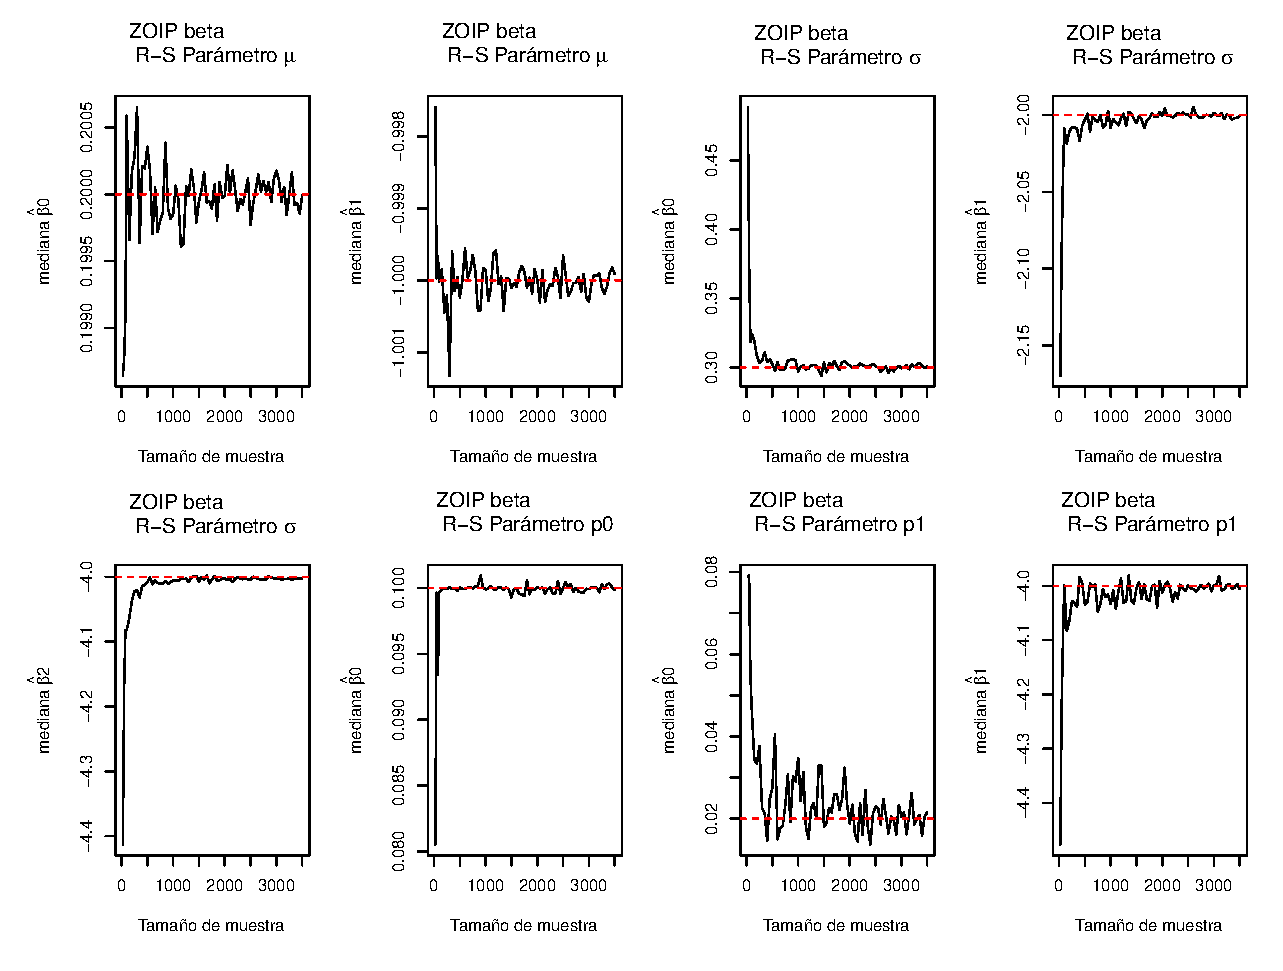
\includegraphics[scale=0.5]{Converg_RS.eps}	
		\caption{Simulaci\'{o}n de un modelo de regresi\'{o}n ZOIP-beta para la parametricazion R-S con diferentes valores de $n$.}
		\label{Simu_RS}
	\end{center}
\end{figure}

En la figura \ref{Simu_RS} se describen los valores estimados para diferentes valores de tama\~{n}o de muestra, cuando se elige realizar una regresi\'{o}n ZOIP-beta con parametrizaci\'{o}n de \cite{Stasinopoulos2}, en ella se ve como todos los par\'{a}metros estimados oscilan alrededor del valor real del par\'{a}metro que es representado por la l\'{\i}nea roja, sin embargo, se nota como unos par\'{a}metros tienen una oscilaci\'{o}n mayor que otros, como es el caso de los par\'{a}metros de intercepto de la media y el del par\'{a}metro de inflaci\'{o}n de unos, asociada a $p_1$. Los de m\'{a}s par\'{a}metros convergen r\'{a}pidamente a sus valores reales, como los par\'{a}metros que representan la variabilidad ($\sigma$) y el par\'{a}metro de $p_0$.\\

\begin{figure}
	\begin{center}
		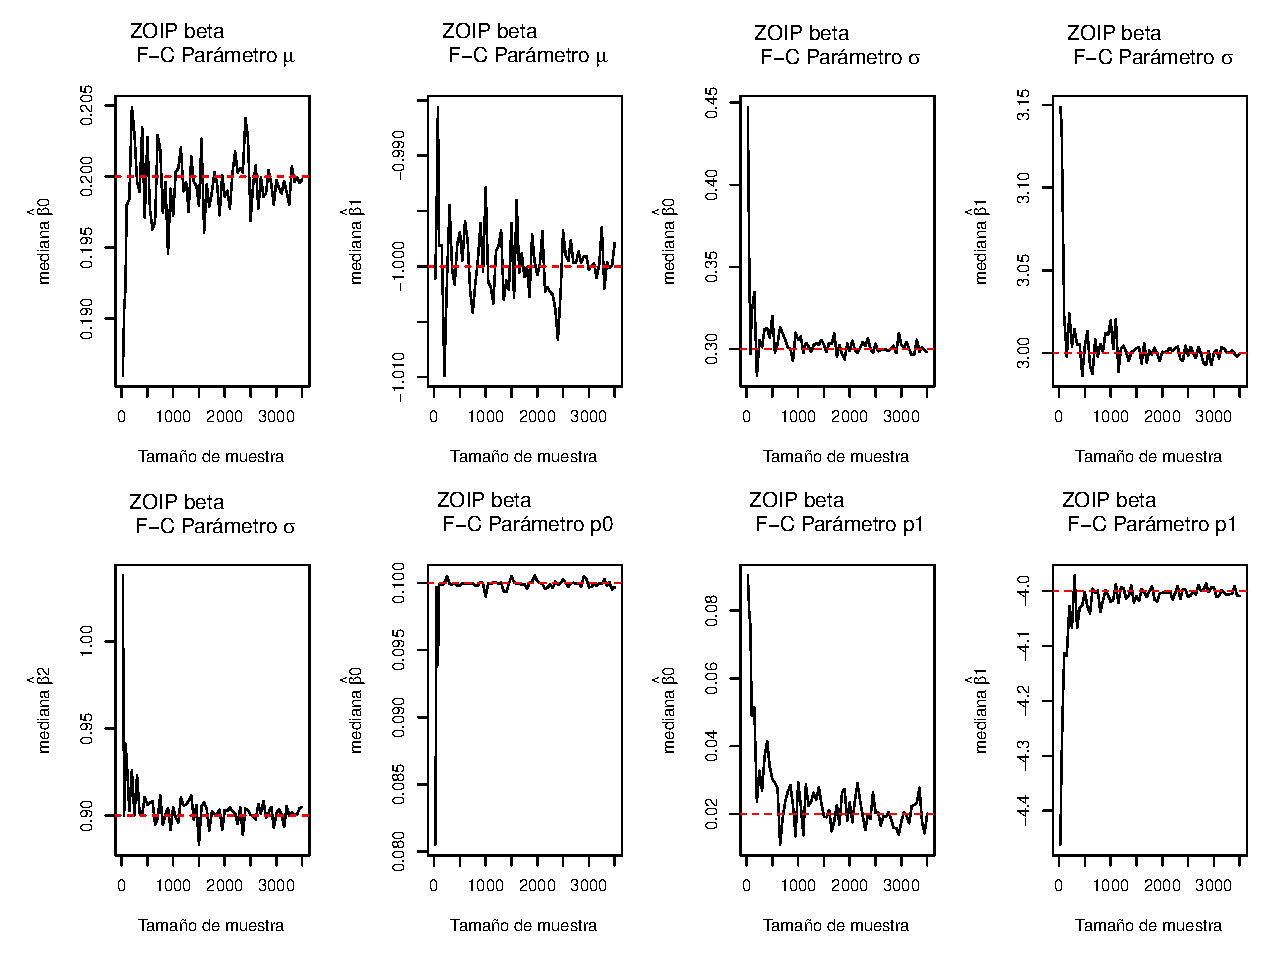
\includegraphics[scale=0.5]{Converg_FC.eps}	
		\caption{Simulaci\'{o}n de un modelo de regresi\'{o}n ZOIP-beta para la parametricazion F-C con diferentes valores de $n$.}
		\label{Simu_FC}
	\end{center}
\end{figure}

En la figura \ref{Simu_FC} se describen los valores estimados para diferentes tama\~{n}os de muestra, cuando se elige realizar una regresi\'{o}n ZOIP-beta con parametrizaci\'{o}n de \cite{Ferrari2}, en dicha figura se nota como la estimaci\'{o}n de los par\'{a}metros asociados con la media tienen una oscilaci\'{o}n mayor que los dem\'{a}s par\'{a}metros, sin embargo, en todos los par\'{a}metros se obsserva como a medida que el tama\~{n}o de muestra es m\'{a}s grande la oscilaci\'{o}n de los par\'{a}metros es menor y van convergiendo satisfactoriamente a sus valores reales.\\

\begin{figure}
	\begin{center}
		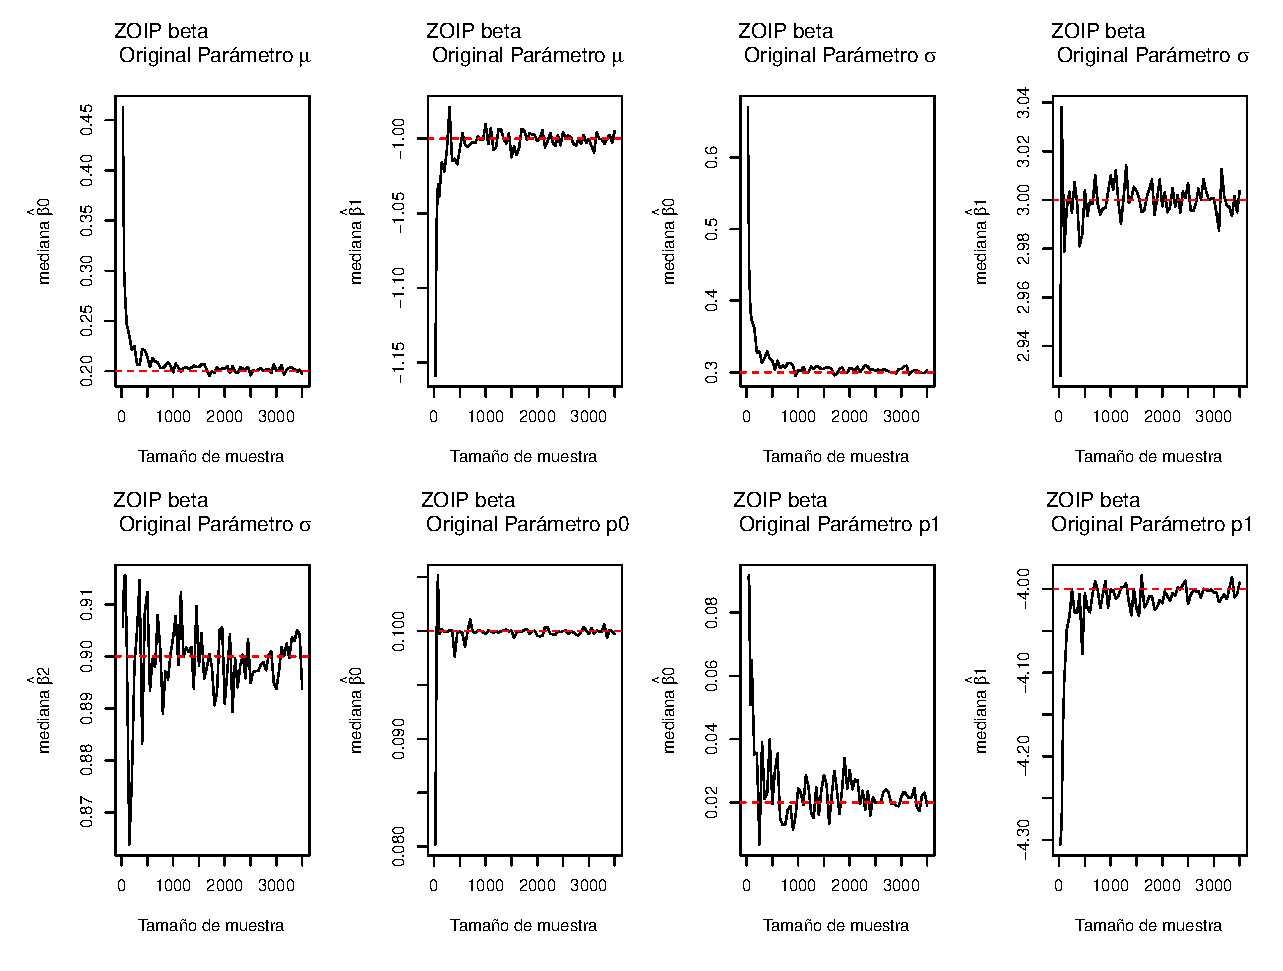
\includegraphics[scale=0.5]{Converg_Ori.eps}	
		\caption{Simulaci\'{o}n de un modelo de regresi\'{o}n ZOIP-beta para la parametricazion original con diferentes valores de $n$.}
		\label{Simu_Ori}
	\end{center}
\end{figure}

En la figura \ref{Simu_Ori} se describen los valores estimados para diferentes tama\~{n}os de muestra, cuando se elige realizar una regresi\'{o}n ZOIP-beta con parametrizaci\'{o}n original, se puede ver como con los valores del escenario de simulaci\'{o}n elegidos, se obtiene una distribuci\'{o}n ZOIP con mayor variabilidad, por lo que los valores de los par\'{a}metros asociados a $\sigma$ tienen una mayor oscilaci\'{o}n, sin embargo, este oscila solo en un 0.01 de sus unidades, lo que no es preocupante. Por otra parte, se observa como el par\'{a}metro de intercepto del par\'{a}metro de inflaci\'{o}n de unos ($p_1$) si oscila mucho m\'{a}s ya que este tiene una desviaci\'{o}n est\'{a}ndar de 0.04 en promedio, pero se observa como a trav\'{e}s de que el tama\~{n}o de muestra es mayor la oscilaci\'{o}n va dis\-mi\-nu\-yen\-do, por lo que se sospecha que se necesita un mayor tama\~{n}o de muestra para que esta converja con mayor satisfacci\'{o}n.\\

\begin{figure}
	\begin{center}
		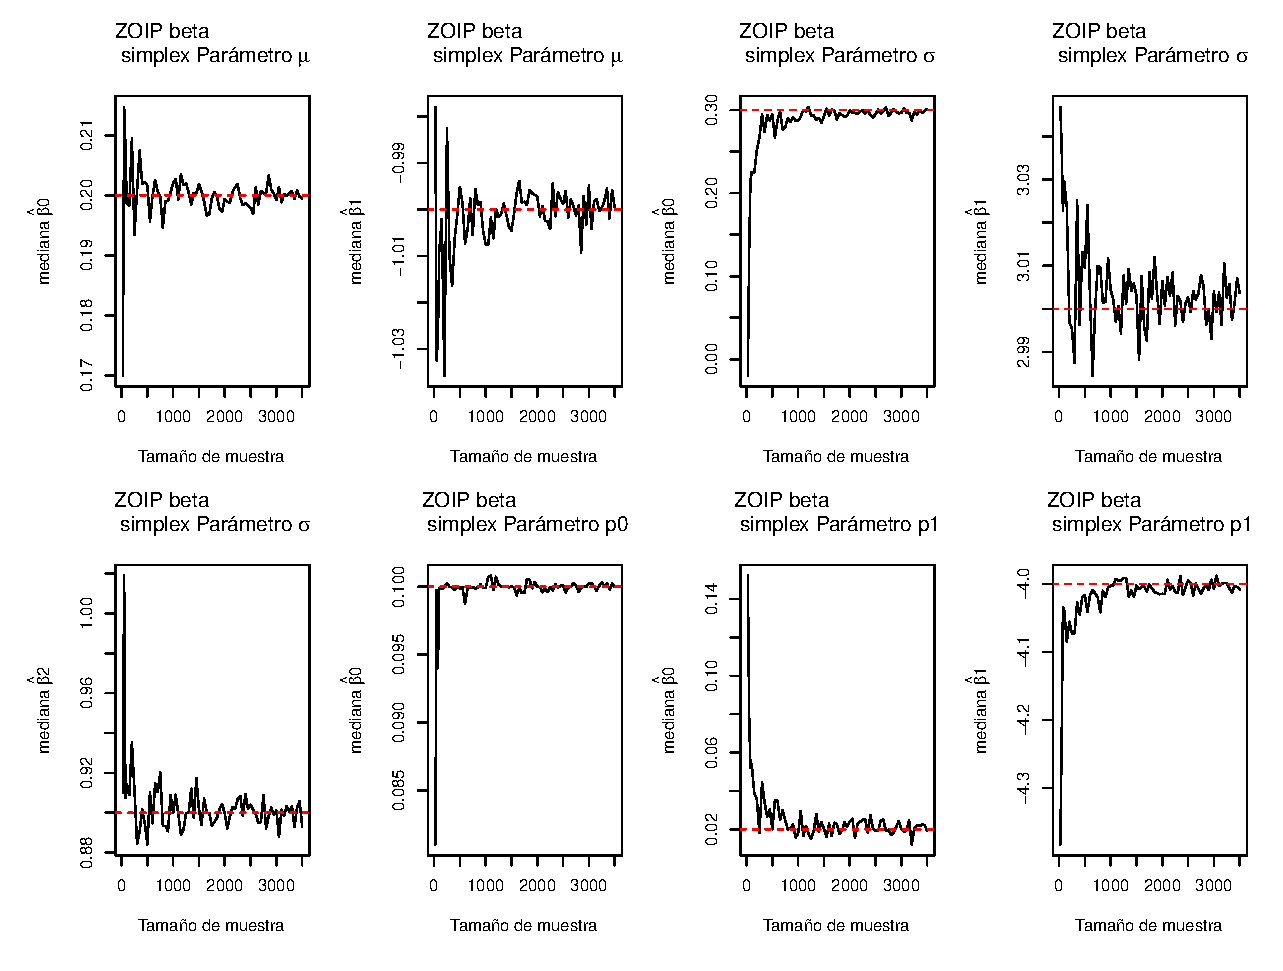
\includegraphics[scale=0.5]{Converg_Simplex.eps}	
		\caption{Simulaci\'{o}n de un modelo de regresi\'{o}n ZOIP-simplex con diferentes valores de $n$.}
		\label{Simu_simplex}
	\end{center}
\end{figure}

En la figura \ref{Simu_simplex} se describen los valores estimados para diferentes tama\~{n}os de muestra, cuando se elige realizar una regresi\'{o}n ZOIP-simplex, Se nota como todos los par\'{a}metros oscilan alrededor de los valores verdaderos y como estas oscilaciones se van reduciendo a trav\'{e}s de que el tama\~{n}o de muestra crece, sin embargo, unos par\'{a}metros toman mayor tiempo de convergencia como es el par\'{a}metro $\beta_1$ asociado al par\'{a}metro de dispersi\'{o}n ($\sigma$).\\



\begin{table}[!hbt]
{\scriptsize
\begin{center}
\begin{tabular}{|c|cc|ccc|c|cc|}\hline
\multirow{2}{*}{Familia} & \multicolumn{2}{|c|}{$\mu$} & \multicolumn{3}{|c|}{$\sigma$} & $p_0$ & \multicolumn{2}{|c|}{$p_1$} \\ \cline{2-9}
& $\hat{\beta}_0$& $\hat{\beta}_1$& $\hat{\beta}_0$& $\hat{\beta}_1$& $\hat{\beta}_2$& $\hat{\beta}_0$ & $\hat{\beta}_0$ & $\hat{\beta}_1$ \\ \hline \hline
R-S & 1.25 & 0.32 & 1.45 & 2.55 & 1.38 & 4.86 & 383.09 & 4.88 \\ 
F-C & 14.22 & 3.96 & 22.21 & 2.9 & 10.14 & 4.86 & 91.21 & 4.88 \\
original & 22.34 & 8.03 & 22.55 & 3.62 & 8.69 & 4.84 & 90.58 & 4.96 \\
simplex & 13.93 & 5.89 & 24.49 & 3.11 & 11.01 & 4.85 & 91.15 & 4.81 \\ \hline
\end{tabular}
\caption{Mediana del MAPE (Error porcentual absoluto medio) en porcentaje para los diferentes parametros en las diferentes parametrizaciones.}
\label{MAPE}
\end{center}
}
\end{table}

En la tabla \ref{MAPE} se muestra la mediana del MAPE de los diferentes par\'{a}metros regresores para cada posible caso de la distribuci\'{o}n o parametrizaci\'{o}n de la distribuci\'{o}n ZOIP, en dicha tabla se nota como el MAPE en los interceptos de cualquier regresi\'{o}n asociada a los par\'{a}metros de la distribuci\'{o}n ZOIP son un poco m\'{a}s grandes que los dem\'{a}s par\'{a}metros regresores de cada regresi\'{o}n, adem\'{a}s se comete un MAPE m\'{a}s grande en las regresiones asociadas a todos los par\'{a}metros de inflaci\'{o}n, esto nos permite concluir que hallar los par\'{a}metros verdaderos en los par\'{a}metros de inflaci\'{o}n es un poco m\'{a}s dif\'{\i}cil que en los par\'{a}metros de localizaci\'{o}n y escala como lo son $\mu$ y $\sigma$, esto se debe a que se posee una menor cantidad de datos en cero y uno, en este escenario de simulaci\'{o}n elegido. Por otro lado, el intercepto asociado a la regresi\'{o}n del par\'{a}metro de inflaci\'{o}n de los unos posee un MAPE muy grande, por lo que nos permite concluir que a pesar de que los diferentes par\'{a}metros estimados en la simulaci\'{o}n oscilan alrededor del valor real este todav\'{\i}a tiene una variabilidad muy grande por lo que hace que este MAPE sea grande y el par\'{a}metro no haya convergido con un tama\~{n}o de muestra de 3500.\\

\begin{figure}
	\begin{center}
		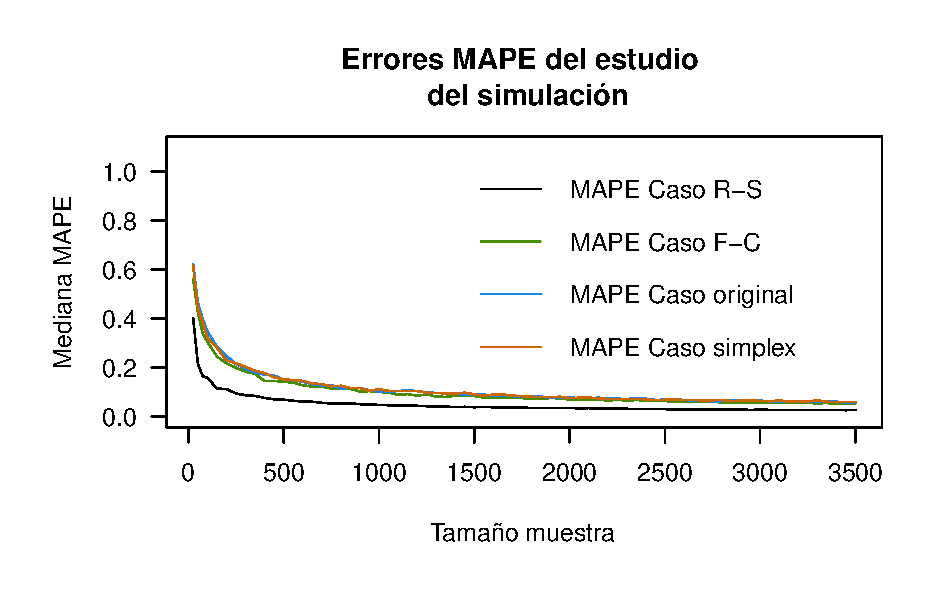
\includegraphics[scale=0.6]{MAPE_gnral.eps}	
		\caption{Mape (Error porcentual absoluto medio) para modelo de regresion ZOIP simulado para distintas parametrizaciones y valores de $n$.}
		\label{Mape_gnrl}
	\end{center}
\end{figure}

En la figura \ref{Mape_gnrl} se muestra la mediana del MAPE de la mediana del MAPE de todos los par\'{a}metros asociados a cada parametrizaci\'{o}n y distribuci\'{o}n para diferentes tama\~{n}os de muestra, en ella se evidencia como el caso de la regresi\'{o}n ZOIP-beta con parametrizaci\'{o}n \cite{Stasinopoulos2} tiene un MAPE menor, donde este tiene asociados unos par\'{a}metros distintos con una distribuci\'{o}n ZOIP con menor variabilidad, por lo que no es del todo comparable con las dem\'{a}s parametrizaciones y distribuciones, se nota un MAPE menor al $20\%$ a partir de un tama\~{n}o de muestra mayor a 500, por lo que se puede concluir que con un tama\~{n}o de muestra mayor a 500 el modelo tendr\'{a} un MAPE aceptable para la estimaci\'{o}n de todos los par\'{a}metros de la regresi\'{o}n ZOIP, sin embargo, esto siempre depender\'{a} de la variabilidad que posean los datos.

\subsection{Datos reales}

En una entidad financiera tiene gran importancia conocer el comportamiento del porcentaje de utilizaci\'{o}n de las tarjetas de cr\'{e}dito (tdc), con el fin de conocer el comportamiento de la cartera de tarjeta de cr\'{e}dito, adem\'{a}s de detectar los diferentes factores que pueden afectar este tipo de cartera. Se define a $y$ como el porcentaje de uso de una tdc, es de notar que $y$ se encuentra entre cero y uno, pero adicional es normal que se tengan tdc que no sean utilizadas ($y=0$) y tdc que est\'{a}n utilizadas en la totalidad de su cupo asignado ($y=1$), por lo que se trata a $y$ como una variable aleatoria perteneciente a datos proporcionales inflados con ceros y unos, es decir $y$ puede ser explicada a partir de una distribuci\'{o}n ZOIP. Se tiene un total de 9206 tarjetas de cr\'{e}dito. Se quiere estudiar el impacto de algunas variables sobre el porcentaje de utilizaci\'{o}n de una tdc, para ello se busca ajustar un modelo de regresi\'{o}n ZOIP mediante la funci\'{o}n \code{RM.ZOIP} del paquete \pkg{ZOIP} de \proglang{R}, que permita explicar el comportamiento del porcentaje de utilizaci\'{o}n de una tdc mediante las siguientes tres variables, \textsl{Score:} variable entre cero y 1000 que para nuestro caso se cambiara de escala entre cero y uno, est\'{a} explica la calificaci\'{o}n del comportamiento de pago del cliente asociada a la tdc, que pertenece a la entidad financiera, donde cero es la peor calificacion y uno un comportamiento de pago ideal; \textsl{Prom Cuotas:} se define como el promedio de cantidad de cuotas al que ha diferido sus compras en los \'{u}ltimos seis meses; \textsl{Cupo tdc Entidad:} es el cupo total asignado a la tdc, esta ser\'{a} tratada como el logaritmo de su cupo m\'{a}s uno, para una mayor estabilidad de su varianza.\\

En el modelo de regresi\'{o}n ZOIP se deben definir cuatro diferentes modelos de regresi\'{o}n para ser ajustados, de tal forma que nos permita ver el efecto de las variables descritas anteriormente sobre cada uno de los par\'{a}metros de la distribuci\'{o}n ZOIP, adicionalmente dependiendo de la parametrizaci\'{o}n o distribuci\'{o}n que se est\'{e} utilizando, se debe utilizar una funci\'{o}n enlace adecuada para cada regresi\'{o}n, en las ecuaciones dadas en \eqref{A_eq_reg} se pueden ver los modelos de regresi\'{o}n a aplicar en cada par\'{a}metro, en estas ecuaciones se ve que dependen de una funci\'{o}n enlace $h(\cdot)$, en la tabla \ref{T_F_enlace2} se muestran las diferentes funciones enlaces adecuadas para cada par\'{a}metro dependiendo de la distribuci\'{o}n escogida y/o la parametrizaci\'{o}n.\\

Si $y_{i} \sim ZOIP(\mu_{i},\sigma_{i},p_{0i}, p_{1i}),$

\begin{equation}
\begin{split}
&h_1(\mu_{i})=\beta_0+\beta_1 x_{1i}+\beta_2 x_{2i}+\beta_3 x_{3i},\\
&h_2(\sigma_{i})=\beta_0+\beta_1 x_{1i}+\beta_2 x_{2i}+\beta_3 x_{3i},\\
&h_3(p_{0i})=\beta_0+\beta_1 x_{1i}+\beta_2 x_{2i}+\beta_3 x_{3i},\\
&h_4(p_{1i}) =\beta_0+\beta_1 x_{1i}+\beta_2 x_{2i}+\beta_3 x_{3i},
\end{split}
\label{A_eq_reg}
\end{equation}

donde $y_i$ es porcentaje de utilizacion de la i-esima tdc, $x_{1i}$: es el valor del score del i-esimo individuo asociada a la tarjeta de cr\'{e}dito, $x_{2i}$: es valor del promedio de cuotas al que difiere sus compras de la i-esima tarjeta de cr\'{e}dito, $x_{3i}$: es el valor del cupo otorgado de la i-esima tarjeta de cr\'{e}dito. 

\begin{table}[!hbt]
{\scriptsize
\begin{center}
\begin{tabular}{|c|c|c|}\hline
Familia & Par\'{a}metro & $h(\cdot)$ \\ \hline
\multirow{4}{*}{R-S} & $\mu$ & Logit \\
 & $\sigma$ & Logit \\
 & $p_0$ & Logit \\
 & $p_1$ & Logit \\ \hline

\multirow{4}{*}{F-C} & $\mu$ & Logit \\
 & $\sigma$ & Log. \\
 & $p_0$ & Logit \\
 & $p_1$ & Logit \\ \hline

\multirow{4}{*}{original} & $\mu$ & Log. \\
 & $\sigma$ & Log. \\
 & $p_0$ & Logit \\
 & $p_1$ & Logit \\ \hline

\multirow{4}{*}{simplex} & $\mu$ & Logit \\
 & $\sigma$ & Log. \\
 & $p_0$ & Logit \\
 & $p_1$ & Logit \\ \hline

\end{tabular}
\caption{Funciones de enlace adecuadas para cada par\'{a}metro, seg\'{u}n su distribuci\'{o}n y/o parametrizaci\'{o}n para el modelo de regresi\'{o}n ZOIP en el porcentaje de utilizaci\'{o}n de una tdc.}
\label{T_F_enlace2}
\end{center}
}
\end{table}

En las ecuaciones dadas en \eqref{A_eq_reg} se puede ver como los par\'{a}metros $\mu$, $\sigma$, $p_0$, $p_1$  ser\'{a}n explicados por las variables score, cupo asignado a su tdc y el promedio al que difiere sus compras, bajo estas ecuaciones podemos observar como se explica el porcentaje utilizaci\'{o}n de una tdc, la variabilidad de este porcentaje de utilizaci\'{o}n, el por que un cliente no llega a utilizar nunca su tdc y adicional y contrariamente a lo anterior, por que un cliente utiliza la total capacidad de su tdc.\\

\begin{table}[!hbt]
{\scriptsize
\begin{center}
\begin{tabular}{|c|c|c|ccc|c|c|}\hline
Familia & Par\'{a}metro & $\beta$'s & Estimaci\'{o}n & Error est\'{a}ndar & Valor P & Log-Verosimilitud & Iteraciones \\ \hline \hline
\multirow{12}{*}{R-S} & \multirow{4}{*}{$\mu$} & $\hat{\beta}_0$ & -0.046	&0.050	&0.3618 & \multirow{12}{*}{-5414.738} & \multirow{12}{*}{125}  \\
& & $\hat{\beta}_1$ & -0.354	&0.107	&0.0009 & &\\
& & $\hat{\beta}_2$ & 0.022	&0.002	&$<2.2e^{-16}$ & & \\
& & $\hat{\beta}_3$ & -0.025	&0.009	&0.0074 & & \\ \cline{2-6}
& \multirow{4}{*}{$\sigma$} & $\hat{\beta}_0$ & 0.822	&0.038	&$<2.2e^{-16}$  & &\\
& & $\hat{\beta}_1$ & -0.197	&0.078	&0.0114  & &\\
& & $\hat{\beta}_2$ & -0.006	&0.002	&0.0013  & &\\
& & $\hat{\beta}_3$ & -0.003	&0.007	&0.6741  & &\\ \cline{2-6}
& \multirow{4}{*}{$p_0$} & $\hat{\beta}_0$ & -1.496	&0.101	&$<2.2e^{-16}$  & &\\
& & $\hat{\beta}_1$ & 0.724	&0.185	&$8.87e^{-5}$  & &\\
& & $\hat{\beta}_2$ & -0.153	&0.009	&$<2.2e^{-16}$  & &\\
& & $\hat{\beta}_3$ & 0.002	&0.015	&0.1243  & &\\ \cline{2-6}
& \multirow{4}{*}{$p_1$} & $\hat{\beta}_0$ &-1.480	&0.095	&$<2.2e^{-16}$  & &\\
& & $\hat{\beta}_1$ & -0.630	&0.254	&0.0132  & &\\
& & $\hat{\beta}_2$ & 0.011	&0.006	&0.0666  & &\\
& & $\hat{\beta}_3$ & -0.069	&0.022	&0.0022  & &\\ \hline

\end{tabular}
\caption{Parametros regresores estimados de un modelo de regresi\'{o}n ZOIP-beta con parametrizaci\'{o}n Rigby y Stasinopoulos (2005) en el porcentaje de utilizaci\'{o}n de una tdc.}
\label{T_Apli_CC_RS}
\end{center}
}
\end{table}


\begin{table}[!hbt]
{\scriptsize
\begin{center}
\begin{tabular}{|c|c|c|ccc|c|c|}\hline
Familia & Par\'{a}metro & $\beta$'s & Estimaci\'{o}n & Error est\'{a}ndar & Valor P & Log-Verosimilitud & Iteraciones \\ \hline \hline
\multirow{12}{*}{F-C} & \multirow{4}{*}{$\mu$} & $\hat{\beta}_0$ & -0.045	&0.050	&0.3667  & \multirow{12}{*}{-5414.605} & \multirow{12}{*}{105} \\
& & $\hat{\beta}_1$ & -0.354	&0.107	&0.0009   & &\\
& & $\hat{\beta}_2$ & 0.022	&0.002	&$<2.2e^{-16}$   & &\\
& & $\hat{\beta}_3$ & -0.025	&0.009	&0.0074   & &\\ \cline{2-6}
& \multirow{4}{*}{$\sigma$} & $\hat{\beta}_0$ & 0.068	&0.045	&0.1286   & &\\
& & $\hat{\beta}_1$ & 0.238	&0.094	&0.0117   & &\\
& & $\hat{\beta}_2$ & 0.007	&0.002	&0.0012   & &\\
& & $\hat{\beta}_3$ & 0.003	&0.008	&0.6854   & &\\ \cline{2-6}
& \multirow{4}{*}{$p_0$} & $\hat{\beta}_0$ & -1.496	&0.101	&$<2.2e^{-16}$  & &\\
& & $\hat{\beta}_1$ & 0.724	&0.185	&$8.87e^{-5}$  & &\\
& & $\hat{\beta}_2$ & -0.153	&0.009	&$<2.2e^{-16}$  & &\\
& & $\hat{\beta}_3$ & 0.002	&0.015	&0.1243  & &\\ \cline{2-6}
& \multirow{4}{*}{$p_1$} & $\hat{\beta}_0$ &-1.480	&0.095	&$<2.2e^{-16}$  & &\\
& & $\hat{\beta}_1$ & -0.630	&0.254	&0.0132  & &\\
& & $\hat{\beta}_2$ & 0.011	&0.006	&0.0666  & &\\
& & $\hat{\beta}_3$ & -0.069	&0.022	&0.0022  & &\\ \hline

\end{tabular}
\caption{Parametros regresores estimados de un modelo de regresi\'{o}n ZOIP-beta con parametrizaci\'{o}n Ferrari y Cribari-Neto (2004) en el porcentaje de utilizaci\'{o}n de una tdc.}
\label{T_Apli_CC_FC}
\end{center}
}
\end{table}


\begin{table}[!hbt]
{\scriptsize
\begin{center}
\begin{tabular}{|c|c|c|ccc|c|c|}\hline
Familia & Par\'{a}metro & $\beta$'s & Estimaci\'{o}n & Error est\'{a}ndar & Valor P & Log-Verosimilitud & Iteraciones \\ \hline \hline
\multirow{12}{*}{original} & \multirow{4}{*}{$\mu$} & $\hat{\beta}_0$ & -0.649	&0.048	&$<2.2e^{-16}$  & \multirow{12}{*}{-5415.386} & \multirow{12}{*}{121} \\
& & $\hat{\beta}_1$ & 0.035	&0.103	&0.7311   & &\\
& & $\hat{\beta}_2$ & 0.019	&0.002	&$<2.2e^{-16}$   & &\\
& & $\hat{\beta}_3$ & -0.011	&0.009	&0.2267 & & \\ \cline{2-6}
& \multirow{4}{*}{$\sigma$} & $\hat{\beta}_0$ & -0.611	&0.054	&$<2.2e^{-16}$   & &\\
& & $\hat{\beta}_1$ & 0.397	&0.111	&0.0003   & &\\
& & $\hat{\beta}_2$ & -0.002	&0.003	&0.4724   & &\\
& & $\hat{\beta}_3$ & 0.015	&0.010	&0.1456   & &\\ \cline{2-6}
& \multirow{4}{*}{$p_0$} & $\hat{\beta}_0$ & -1.496	&0.101	&$<2.2e^{-16}$  & &\\
& & $\hat{\beta}_1$ & 0.724	&0.185	&$8.87e^{-5}$  & &\\
& & $\hat{\beta}_2$ & -0.153	&0.009	&$<2.2e^{-16}$  & &\\
& & $\hat{\beta}_3$ & 0.002	&0.015	&0.1243  & &\\ \cline{2-6}
& \multirow{4}{*}{$p_1$} & $\hat{\beta}_0$ &-1.480	&0.095	&$<2.2e^{-16}$  & &\\
& & $\hat{\beta}_1$ & -0.630	&0.254	&0.0132  & &\\
& & $\hat{\beta}_2$ & 0.011	&0.006	&0.0666  & &\\
& & $\hat{\beta}_3$ & -0.069	&0.022	&0.0022  & &\\ \hline


\end{tabular}
\caption{Parametros regresores estimados de un modelo de regresi\'{o}n ZOIP-beta con parametrizaci\'{o}n original en el porcentaje de utilizaci\'{o}n de una tdc.}
\label{T_Apli_CC_Ori}
\end{center}
}
\end{table}


\begin{table}[!hbt]
{\scriptsize
\begin{center}
\begin{tabular}{|c|c|c|ccc|c|c|}\hline
Familia & Par\'{a}metro & $\beta$'s & Estimaci\'{o}n & Error est\'{a}ndar & Valor P & Log-Verosimilitud & Iteraciones \\ \hline \hline
\multirow{12}{*}{simplex} & \multirow{4}{*}{$\mu$} & $\hat{\beta}_0$ & 0.180	&0.050	&0.0003  & \multirow{12}{*}{-22385.78} & \multirow{12}{*}{117} \\
& & $\hat{\beta}_1$ & -3.890	&0.206	&$<2.2e^{-16}$   & &\\
& & $\hat{\beta}_2$ & 0.166	&0.004	&$<2.2e^{-16}$   & &\\
& & $\hat{\beta}_3$ & -0.128	&0.019	&$5.85e^{-12}$   & &\\ \cline{2-6}
& \multirow{4}{*}{$\sigma$} & $\hat{\beta}_0$ & 11.59	&0.062	&$<2.2e^{-16}$   & &\\
& & $\hat{\beta}_1$ & 0.063	&0.240	&0.7918   & &\\
& & $\hat{\beta}_2$ & 0.134	&0.004	&$<2.2e^{-16}$  & &\\
& & $\hat{\beta}_3$ & 0.344	&0.023	&$<2.2e^{-16}$   & &\\ \cline{2-6}
& \multirow{4}{*}{$p_0$} & $\hat{\beta}_0$ & -1.496	&0.101	&$<2.2e^{-16}$  & &\\
& & $\hat{\beta}_1$ & 0.724	&0.185	&$8.87e^{-5}$  & &\\
& & $\hat{\beta}_2$ & -0.153	&0.009	&$<2.2e^{-16}$  & &\\
& & $\hat{\beta}_3$ & 0.002	&0.015	&0.1243  & &\\ \cline{2-6}
& \multirow{4}{*}{$p_1$} & $\hat{\beta}_0$ &-1.480	&0.095	&$<2.2e^{-16}$  & &\\
& & $\hat{\beta}_1$ & -0.630	&0.254	&0.0132  & &\\
& & $\hat{\beta}_2$ & 0.011	&0.006	&0.0666  & &\\
& & $\hat{\beta}_3$ & -0.069	&0.022	&0.0022  & &\\ \hline

\end{tabular}
\caption{Parametros regresores estimados de un modelo de regresi\'{o}n ZOIP-simplex en el porcentaje de utilizaci\'{o}n de una tdc.}
\label{T_Apli_CC_Sim}
\end{center}
}
\end{table}

En las tablas \ref{T_Apli_CC_RS}, \ref{T_Apli_CC_FC}, \ref{T_Apli_CC_Ori}, \ref{T_Apli_CC_Sim} se tiene informaci\'{o}n sobre como las covariables influyen en los par\'{a}metros de los cuatro diferentes modelos ajustados de la regresi\'{o}n ZOIP, primero se puede ver que al modelar el par\'{a}metro de la media, es decir, el porcentaje medio de utilizaci\'{o}n de la tdc, la variable regresora score afecta de manera negativa y significativa en cada uno de los modelos ajustados, excepto en el mo\-de\-lo con parametrizaci\'{o}n original, en el cual el par\'{a}metro no dio significativo, esto nos indica que a un mejor comportamiento de pago, menos utilizaci\'{o}n de la tdc, sobre el par\'{a}metro del promedio de cuotas diferidas vemos como el par\'{a}metro $\beta_2$ sin excepci\'{o}n alguna en todos los modelos es la variable m\'{a}s significativa que permite explicar la proporci\'{o}n media de la utilizaci\'{o}n de una tdc, esto nos indica que a medida que los clientes difieren a mayores cuotas sus compras con la tdc estar\'{a}n utilizando m\'{a}s su tdc, algo muy l\'{o}gico, desde el punto de vista del problema; ahora el par\'{a}metro $\beta_3$ asociado al cupo de su tdc tiene un efecto negativo aunque no muy significativo sobre la variable respuesta, lo cual indicar\'{\i}a que a mayor cupo en su tdc un poco menos de utilizaci\'{o}n de la tdc estar\'{a} acompa\~{n}ado.\\

Al analizar el efecto de la variabilidad de la utilizaci\'{o}n de las tdc, se observa como el par\'{a}metro de score tiene un efecto positivo sobre la precisi\'{o}n de la utilizaci\'{o}n de la tdc, en el modelo ZOIP-beta parametrizaci\'{o}n \cite{Stasinopoulos2} este efecto parece ser negativo, pero $\sigma$ al estar representando la dispersi\'{o}n y no la precisi\'{o}n, estar\'{\i}a dando un efecto positivo sobre la precisi\'{o}n, por lo tanto a mejor comportamiento de pago la utilizaci\'{o}n de la tdc ser\'{a}n m\'{a}s parecidas entre los individuos, cabe resaltar que $\beta_1$ no es significativo en el modelo simplex. Adem\'{a}s el par\'{a}metro $\beta_3$ asociado al cupo de la tdc no influye sobre la variabilidad en ninguno de los modelos propuestos, excepto en modelo de regresi\'{o}n ZOIP-simplex que tiene un efecto positivo sobre la variabilidad de los porcentajes de utilizaci\'{o}n de las tdc.\\

Por otra parte el efecto de que alguien no utilice su tdc es exactamente igual en los cuatro modelos propuestos, esto por la metodolog\'{\i}a de estimaci\'{o}n de m\'{a}xima verosimilitud, y se puede observar como el comportamiento de pago y la cantidad de cuotas a las que se difiere las compras el cliente afectan de manera significativa la no utilizaci\'{o}n de las tdc. Adem\'{a}s es de resaltar que si los clientes no difieren a grandes cuotas sus compras y su comportamiento de pago es muy bueno estos clientes tendr\'{a}n mayor probabilidad de no utilizar para nada las tdc.\\

En el porcentaje de utilizaci\'{o}n global de la tdc, vemos como las tres covariables incluidas en el modelo afectan de manera significativa la utilizaci\'{o}n por completo de la tdc y vemos como la variable que es m\'{a}s significativa es el cupo de las tdc y que este tiene un efecto negativo sobre la probabilidad de utilizar por completo mi tdc, lo que me indica que a mayor cupo menor probabilidad de utilizar por completo de mi tdc (efecto que hab\'{\i}amos evidenciado en la explicaci\'{o}n de la utilizaci\'{o}n media de las tdc), el mismo efecto pasa sobre la variable score que me indica que a peor comportamiento de pago m\'{a}s utilizaci\'{o}n la tdc, sin embargo si el cliente difiere a grandes cuotas su compras este tendera a tener una mayor probabilidad de utilizar por completo su tdc. cabe resaltar que el efecto de las covariables sobre la probabilidad de utilizar por completo la tdc es totalmente contrario al efecto causado sobre la probabilidad de no utilizar para nada la tdc, algo l\'{o}gico y esperado.\\

Al analizar el valor de la log-verosimilitud se observa que el mejor modelo de regresi\'{o}n que explica el porcentaje de utilizaci\'{o}n de una tdc en esta entidad financiera es la regresi\'{o}n ZOIP-beta, ya que posee un valor de log-verosimilitud menor que el modelo de regresi\'{o}n ZOIP-simplex, sin embargo no importa la parametrizaci\'{o}n que se tenga en la regresi\'{o}n ZOIP-beta, porque el valor de la log-verosimilitud son significativamente iguales, sin embargo el modelo que requiere menor n\'{u}mero de iteraciones para ser ajustado es la regresi\'{o}n ZOIP-beta parametrizaci\'{o}n \cite{Ferrari2} seguido por la parametrizaci\'{o}n original y por \'{u}ltimo la parametrizacion de \cite{Stasinopoulos2}.


%%%%%%%%%%%%%%%%%%%%%%%%%%%%%%%%%%%%%%%%%%%%%%%%%%%%%%%%%%%%%%%%%%%%%%%%%%%%%%%%%%%%%%%%%%%%%%%%%%%%%%%%%%%%%%%%%%%%%%%%%%%%%%%%%%%%%%%%%%%%%%%%%%%%%%%%%%%%%%%%%%

\section{Conclusi\'{o}n}

El modelo de regresi\'{o}n ZOIP, es un modelo de regresi\'{o}n de efectos fijos que es desarrollado bajo la distribuci\'{o}n ZOIP y el cual se encarga de encontrar las covariables o factores que m\'{a}s influyen en una variable respuesta cuya distribuci\'{o}n asociada es una distribuci\'{o}n ZOIP. La estimaci\'{o}n del efecto de las covariables sobre la variable respuesta se realiza mediante m\'{a}xima verosimilitud, dicha maximizaci\'{o}n de la verosimilitud no tiene una soluci\'{o}n cerrada anal\'{\i}ticamente, por lo que se realiza computacionalmente y el paquete \pkg{ZOIP} de \proglang{R} da una soluci\'{o}n a esto. Seg\'{u}n los estudios de simulaci\'{o}n realizados en este trabajo, las estimaciones convergen con un tama\~{n}o de muestra moderado a sus valores reales; aunque en ocasiones ocurre que las convergencias de los efectos de las covariables asociadas a los par\'{a}metros de inflaci\'{o}n requieren un mayor n\'{u}mero de muestras para demostrar su convergencia.\\

En el modelo de regresi\'{o}n ZOIP y el paquete \pkg{ZOIP} de \proglang{R} es posible realizar de una manera muy sencilla los principales tipos de regresiones para datos proporciones inflados con ceros y unos que existen, como la regresi\'{o}n simplex y la regresi\'{o}n beta bajo diferentes parametrizaciones, adem\'{a}s el modelo de regresi\'{o}n ZOIP permite realizar ajustes a modelos inflados unilateralmente, es decir, donde solo haya datos proporcionales con valores cero o uno, e incluso realizar un ajuste sobre un modelo de regresi\'{o}n para datos proporcionales sin inflaciones.

